% Presentación del proyecto completo (41 láminas). Compilar dos veces: pdflatex presentacion_proyecto.tex
% Cifras: informe final (docs/6_presentacion/informe_final), resultados del repositorio al 9/11/2026.
\documentclass[aspectratio=169,11pt]{beamer}
% Estilo común de la presentación y del guion (mismos colores que el guion del 6/11/2026)
\usepackage[utf8]{inputenc}
\usepackage[T1]{fontenc}
\usepackage[spanish,es-noshorthands,es-nodecimaldot]{babel}
\usepackage{lmodern}
\usepackage{booktabs,tabularx,array,amsmath,amssymb,bbm}
\usepackage{tikz}
\usetikzlibrary{arrows.meta,positioning,calc,shapes.geometric,decorations.pathreplacing}
\tikzset{bx/.style={draw=#1,fill=#1!8,rounded corners=2mm,minimum width=3.6cm,minimum height=1.5cm,align=center,text width=3.4cm},
  barra/.style={fill=azul!#1,minimum height=0.5cm,anchor=west}}
\usepackage[most]{tcolorbox}
\graphicspath{{figuras/}}

\definecolor{azul}{HTML}{1F5F99}
\definecolor{naranja}{HTML}{DF7A27}
\definecolor{verde}{HTML}{2D8B57}
\definecolor{morado}{HTML}{6D3584}
\definecolor{rojo}{HTML}{C8372D}
\definecolor{gris}{HTML}{5B6770}
\definecolor{grisclaro}{HTML}{F2F3F4}

\usetheme{default}
\setbeamertemplate{navigation symbols}{}
\setbeamercolor{structure}{fg=azul}
\setbeamercolor{frametitle}{fg=white,bg=azul}
\setbeamertemplate{itemize item}{\color{naranja}$\blacktriangleright$}
\setbeamertemplate{itemize subitem}{\color{naranja}\textbullet}
\setbeamertemplate{enumerate item}{\color{azul}\insertenumlabel.}
\setbeamerfont{frametitle}{series=\bfseries,size=\large}

% caja con título de color (como en el guion antiguo)
\newtcolorbox{caja}[2][azul]{enhanced,colback=#1!7,colframe=#1,coltitle=white,
  fonttitle=\bfseries\small,title={#2},boxrule=0.6pt,arc=2mm,left=4pt,right=4pt,top=2pt,bottom=2pt,fontupper=\small}
\newtcolorbox{cajasin}[1][azul]{enhanced,colback=#1!6,colframe=#1!70,boxrule=0.6pt,arc=2mm,left=5pt,right=5pt,top=3pt,bottom=3pt,fontupper=\small}
% cifra grande
\newcommand{\cifra}[3][azul]{\begin{tcolorbox}[enhanced,colback=#1!6,colframe=#1!45,boxrule=0.5pt,arc=1.5mm,halign=center,top=1pt,bottom=1pt,left=2pt,right=2pt]
  {\Large\bfseries\color{black}#2}\\[-1pt]{\footnotesize\color{black!80}#3}\end{tcolorbox}}
\newcommand{\ind}{\mathbbm{1}}

\title{Inundaciones por El Niño costero en Tumbes y Piura}

\setbeamercolor{normal text}{fg=black!85}
\setbeamertemplate{frametitle}{%
  \nointerlineskip\begin{beamercolorbox}[wd=\paperwidth,ht=2.9ex,dp=1.3ex,leftskip=0.9em]{frametitle}%
  \usebeamerfont{frametitle}\insertframetitle\end{beamercolorbox}%
  \vspace{0.6ex}\hspace*{1.6em}{\color{naranja}\rule{\dimexpr\paperwidth-1.6em}{1.2pt}}\vspace{-0.6ex}}
\setbeamertemplate{footline}{\hfill{\color[HTML]{5D6D7E}\scriptsize Inundaciones por El Niño en Tumbes y Piura\quad\insertframenumber/\inserttotalframenumber}\hspace{1.2em}\vspace{1.4ex}}
\newcommand{\parte}[2]{{\setbeamertemplate{footline}{}\setbeamercolor{background canvas}{bg=azul}
  \begin{frame}[plain]\begin{tikzpicture}[remember picture,overlay]
  \node[anchor=west,color=white!85!azul] at ([xshift=2.2em,yshift=0.6em]current page.west) {\normalsize Parte #1};
  \fill[naranja] ([yshift=-1.6em]current page.west) rectangle ([xshift=0.185\paperwidth,yshift=-2.05em]current page.west);
  \node[anchor=west,color=white,font=\Large\bfseries] at ([xshift=0.23\paperwidth,yshift=-1.8em]current page.west) {#2};
  \end{tikzpicture}\end{frame}}}

\begin{document}

% ---------------------------------------------------------------- 1
{\setbeamertemplate{footline}{}
\begin{frame}[plain]
\begin{tikzpicture}[remember picture,overlay]
\fill[azul] (current page.north west) rectangle ([yshift=-0.645\paperheight]current page.north east);
\fill[naranja] ([yshift=-0.645\paperheight]current page.north west) rectangle ([yshift=-0.665\paperheight]current page.north east);
\node[anchor=north west,text width=0.88\paperwidth,color=white,align=left] at ([xshift=2.4em,yshift=-1.6em]current page.north west)
 {{\tiny PROYECTO INTEGRADOR · PROGRAMA DE EXTENSIÓN UNIVERSITARIA CIENCIA DEL DATO · INEI 2026}\\[0.8em]
  {\Large\bfseries Inundaciones por El Niño costero en Tumbes y Piura:\\[0.15em] anticipar emergencias semanas antes}\\[0.8em]
  {\small Probabilidad de emergencia a una y cuatro semanas en cada distrito, fases de aviso y población expuesta según los Censos Nacionales 2025}};
\node[anchor=north west,text width=0.9\paperwidth,align=left] at ([xshift=2.4em,yshift=-0.72\paperheight]current page.north west)
 {\footnotesize\textbf{Equipo:} Christopher Calle, Luz Ángela Mendizábal, Maykol Ramírez y Marcia Shapiama \quad \textbf{Asesor:} Prof. Alexander Quispe\\[0.3em]
  \textbf{Tablero:} maykolramirez.github.io/FENOMENO-PREDI \quad \textbf{Código:} github.com/MaykolRamirez/FENOMENO-PREDI};
\end{tikzpicture}
\end{frame}}

% ---------------------------------------------------------------- 2
\begin{frame}{El problema}
\begin{columns}[T]
\begin{column}{0.56\textwidth}
\begin{itemize}\small
\item Cuando el mar frente a Tumbes y Piura se calienta (\textbf{El Niño costero}), llueve en la costa desértica y los ríos Tumbes, Chira y Piura se desbordan.
\item En \textbf{2017} y \textbf{2023} (ciclón Yaku) el INDECI registró más de \textbf{85 mil} y \textbf{118 mil} viviendas afectadas en estos dos departamentos.
\item En noviembre de 2026 el mar está otra vez muy caliente: Niño 1+2 en \textbf{+5,6 °C}; el ENFEN lo califica como Niño costero de magnitud \textbf{extraordinaria}.
\end{itemize}
\begin{caja}{La pregunta del proyecto}
¿Qué tan probable es que un distrito tenga una emergencia por lluvia o inundación en las \textbf{próximas 1 a 4 semanas}, mejor que su propia historia, y a \textbf{cuántas viviendas y personas} alcanzaría?
\end{caja}
\end{column}
\begin{column}{0.36\textwidth}
\cifra[rojo]{85 960}{viviendas afectadas en 2017 (SINPAD)}
\cifra[rojo]{118 241}{viviendas afectadas en 2023 (SINPAD)}
\cifra[naranja]{+5,6 °C}{Niño 1+2, semana del 2 al 8 de noviembre de 2026 (NOAA)}
\end{column}
\end{columns}
\end{frame}

% ---------------------------------------------------------------- 3
\begin{frame}{Objetivos}
\begin{caja}{Objetivo general}
Estimar, para cada uno de los \textbf{78 distritos} de Tumbes y Piura, la probabilidad de una emergencia por lluvia o inundación en las próximas una a cuatro semanas y la cantidad de viviendas y personas expuestas, para anticipar emergencias durante el Niño costero.
\end{caja}
\vspace{0.3em}
\begin{columns}[T]
\begin{column}{0.48\textwidth}\small\textbf{Objetivos específicos}
\begin{enumerate}\footnotesize
\item Cuantificar viviendas y personas en zona inundable con los Censos Nacionales 2025.
\item Construir un aviso de 1 a 3 días con pronósticos de lluvia y caudal, y probarlo con el pasado.
\item Entrenar y validar un modelo de 1 a 4 semanas y compararlo con referencias simples.
\end{enumerate}
\end{column}
\begin{column}{0.48\textwidth}
\vspace{1.1em}\begin{enumerate}\footnotesize\setcounter{enumi}{3}
\item Calibrar las probabilidades, definir fases de aviso y medir la incertidumbre.
\item Publicar todo en un tablero abierto, reproducible y que se actualiza solo.
\end{enumerate}
\end{column}
\end{columns}
\end{frame}

% ---------------------------------------------------------------- 4
\begin{frame}{La idea en un dibujo: tres tiempos y una base común}
\centering
\begin{tikzpicture}[font=\footnotesize]
\node[bx=azul] (a) at (0,0) {\textbf{1. ANTICIPAR}\\[2pt]Aviso de lluvia y caudal (1–3 días)\\Modelo de probabilidad (1–4 semanas)};
\node[bx=verde] (c) at (4.4,0) {\textbf{2. CONFIRMAR}\\[2pt]Radar Sentinel-1\\(agua vista desde el espacio)};
\node[bx=morado] (d) at (8.8,0) {\textbf{3. COMPROBAR}\\[2pt]SINPAD del INDECI, noticias y Copernicus 2017};
\node[draw=naranja,fill=naranja!10,rounded corners=2mm,minimum width=12.4cm,minimum height=1.1cm,align=center] (e) at (4.4,-2.0)
 {\textbf{BASE COMÚN: EXPOSICIÓN}\\zona inundable (JRC) · Censos Nacionales 2025 · colegios, salud, vías y cultivos};
\draw[-{Latex},thick,gris] (a) -- (c); \draw[-{Latex},thick,gris] (c) -- (d);
\end{tikzpicture}
\par\vspace{1em}\small Todo se muestra en un \textbf{tablero web público} que se actualiza solo: el aviso cada día y el modelo cada lunes.
\end{frame}

\parte{1}{Cómo se construyó}

% ---------------------------------------------------------------- 6
\begin{frame}{Línea de tiempo: de un monitor del mar a un sistema de alerta}
\centering
\begin{tikzpicture}[font=\scriptsize,every node/.append style={font=\tiny}]
\draw[very thick,azul] (0,0) -- (13.4,0);
\foreach \x/\d/\t/\c in {0.9/3 nov/Arranque/azul, 3.2/4 nov/Rigor/azul, 5.5/5 nov/Anticipar/azul, 7.8/6 nov/Cierre del avance/azul, 10.1/7–8 nov/Modelo por plazo/naranja, 12.4/9 nov/Informe final/naranja}{
  \fill[\c] (\x,0) circle (3pt); \node[above=4pt,font=\scriptsize\bfseries] at (\x,0) {\d}; \node[below=4pt,font=\scriptsize\bfseries,color=\c] at (\x,0) {\t};}
\node[text width=2.05cm,align=left,anchor=north,font=\tiny] at (0.9,-0.7) {· Monitor del mar\\· Prueba de fuentes\\· Lluvia, caudal y radar\\· Primer modelo};
\node[text width=2.05cm,align=left,anchor=north,font=\tiny] at (3.2,-0.7) {· Auditoría de cifras\\· Mapa JRC\\· Colegios y salud\\· Validación 2017};
\node[text width=2.05cm,align=left,anchor=north,font=\tiny] at (5.5,-0.7) {· Censo 2025\\· Aviso p95/p99\\· Y del SINPAD\\· Noticias verificadas};
\node[text width=2.05cm,align=left,anchor=north,font=\tiny] at (7.8,-0.7) {· Sexo y edad\\· Centros poblados\\· 78 distritos\\· Presentación};
\node[text width=2.05cm,align=left,anchor=north,font=\tiny] at (10.1,-0.7) {· Probabilidad a 1–4 semanas\\· Test de realidad\\· Calibración y fases};
\node[text width=2.05cm,align=left,anchor=north,font=\tiny] at (12.4,-0.7) {· Intervalos de confianza\\· Prioridad y vulnerabilidad\\· Informe final};
\end{tikzpicture}
\par\vspace{0.8em}\small Empezó como un monitor del mar. Al ver que el riesgo concreto eran las inundaciones, el foco se cerró en Tumbes y Piura. Tras la reunión con el asesor, el modelo pasó de un índice a una \textbf{probabilidad por plazo}.
\end{frame}

% ---------------------------------------------------------------- 7
\begin{frame}{Cómo trabajamos: equipo + asistente de inteligencia artificial}
\begin{columns}[c]
\begin{column}{0.44\textwidth}\centering
\begin{tikzpicture}[font=\scriptsize,n/.style={draw=azul,fill=azul!8,rounded corners=1.5mm,align=center,text width=1.7cm,minimum height=0.8cm}]
\foreach \a/\t [count=\i] in {90/1. Pregunta (equipo),30/2. Probar la fuente,-30/3. Código (IA + revisión),-90/4. Prueba automática,-150/5. Validar vs. dato oficial,150/6. Documentar y publicar}
 \node[n] (n\i) at (\a:1.95) {\t};
\foreach \i/\j in {1/2,2/3,3/4,4/5,5/6,6/1} \draw[-{Latex},gris] (n\i) -- (n\j);
\end{tikzpicture}
\end{column}
\begin{column}{0.52\textwidth}
\begin{caja}{El equipo}
Define las preguntas, conoce el territorio, decide qué entra y qué no, revisa las cifras y consigue los datos (por ejemplo, el Censo 2025 del INEI).
\end{caja}
\begin{caja}[naranja]{El asistente de IA (Claude)}
Busca y prueba fuentes, escribe el código en Python, corre las pruebas, detecta errores y redacta documentos.
\end{caja}
\small\textbf{Regla:} ninguna cifra se publica si no sale de un código que se pueda volver a correr.
\end{column}
\end{columns}
\end{frame}

% ---------------------------------------------------------------- 8
\begin{frame}{El proyecto en números}
\begin{columns}[T]
\begin{column}{0.23\textwidth}\cifra{46}{programas en Python (src/)}\cifra{8 059}{líneas de código}\end{column}
\begin{column}{0.23\textwidth}\cifra{87}{pruebas automáticas}\cifra{6}{tareas automáticas (GitHub Actions)}\end{column}
\begin{column}{0.23\textwidth}\cifra{52}{documentos técnicos}\cifra{15+}{fuentes públicas y oficiales}\end{column}
\begin{column}{0.23\textwidth}\cifra[naranja]{78}{distritos (13 Tumbes, 65 Piura)}\cifra[naranja]{1 200}{semanas de datos (2003–2025)}\end{column}
\end{columns}
\end{frame}

% ---------------------------------------------------------------- 9
\begin{frame}{Arquitectura: cómo viajan los datos hasta el tablero}
\centering
\begin{tikzpicture}[font=\scriptsize,f/.style={draw=gris,fill=grisclaro,rounded corners=1mm,text width=3.0cm,align=center,minimum height=0.42cm,font=\tiny},
 m/.style={draw=azul,fill=azul!8,rounded corners=2mm,text width=2.5cm,align=center,minimum height=1.1cm}]
\foreach \t [count=\i] in {Mar (NOAA),{Lluvia (NASA, Open-Meteo)},Ríos (GloFAS),Radar (Sentinel-1),{Exposición (JRC, Censo)},Emergencias (SINPAD)}
  \node[f] (s\i) at (0,1.9-0.58*\i) {\t};
\node[m] (src) at (4,0.4) {\textbf{src/}\\46 programas Python: descargan y calculan};
\node[m] (gh) at (4,-1.4) {\textbf{GitHub Actions}\\diario (aviso) y lunes (modelo)};
\node[m] (data) at (7.6,0.4) {\textbf{data/}\\datos limpios y resultados};
\node[m] (t) at (7.6,-1.4) {\textbf{tests/}\\87 pruebas: si fallan, no se publica};
\node[draw=naranja,fill=naranja!10,rounded corners=2mm,text width=2.4cm,align=center,minimum height=1.6cm] (w) at (11,-0.5) {\textbf{Tablero web}\\GitHub Pages};
\foreach \i in {1,...,6} \draw[-{Latex},gris] (s\i.east) -- (src.west);
\draw[-{Latex},gris] (gh) -- (src); \draw[-{Latex},gris] (src) -- (data); \draw[-{Latex},gris] (data) -- (t); \draw[-{Latex},gris] (t) -- (w);
\end{tikzpicture}
\par\vspace{0.5em}\footnotesize Si una descarga falla, se queda la última versión válida y la capa se marca como «rezagada». Cada cifra del tablero tiene su fuente y fecha.
\end{frame}

% ---------------------------------------------------------------- 10
\begin{frame}{Las fuentes de datos}
\footnotesize
\begin{tabularx}{\textwidth}{@{}l X l@{}}
\toprule
\textbf{Tema} & \textbf{Fuente} & \textbf{Para qué}\\\midrule
Emergencias & SINPAD del INDECI, 2003–junio 2026 (datos abiertos) & Variable Y\\
Personas y viviendas & Censos Nacionales 2025 (INEI, por manzana y centro poblado) & Exposición\\
Zona inundable & JRC CEMS-GloFAS: crecidas de 1 en 10 y 1 en 100 años (90 m) & Exposición\\
Lluvia & NASA POWER (diaria por distrito); Open-Meteo (pronóstico y últimos días); ERA5 1991–2020 & Modelo y aviso\\
Ríos & GloFAS v4 (caudal diario y pronóstico de 7 días) & Modelo y aviso\\
Mar & NOAA OISST e índice Niño 1+2; comunicados del ENFEN & Modelo\\
Satélite & Sentinel-1 (radar) y Sentinel-2 (fotos), vía Planetary Computer & Confirmar agua\\
Servicios & Colegios (ESCALE), salud (RENIPRESS), vías (OpenStreetMap), pobreza 2018 (INEI) & Exposición y prioridad\\
Validación & Copernicus EMS 2017 (mapa oficial); noticias verificadas & Comprobar\\\bottomrule
\end{tabularx}
\end{frame}

\parte{2}{Exposición: ¿a quién alcanzaría?}

% ---------------------------------------------------------------- 12
\begin{frame}{Zona inundable: escenarios de crecida de 1 en 10 y 1 en 100 años}
\begin{columns}[T]
\begin{column}{0.5\textwidth}\small
El mapa del JRC (Comisión Europea) indica hasta dónde y a qué profundidad llegaría el agua en una crecida que tiene:
\begin{itemize}\small
\item \textbf{10 \%} de probabilidad cada año (1 en 10);
\item \textbf{1 \%} de probabilidad cada año (1 en 100).
\end{itemize}
\begin{cajasin}
$\Pr(\text{al menos una en } n \text{ años}) = 1-(1-p)^n$\\[2pt]
$1-0{,}99^{30} \approx 0{,}26$: un 26 \% en 30 años
\end{cajasin}
\begin{caja}[naranja]{Ojo}
\textbf{Expuesto} = vive dentro de la zona inundable. No equivale a afectado: esa cifra la registra el INDECI.
\end{caja}
\end{column}
\begin{column}{0.46\textwidth}
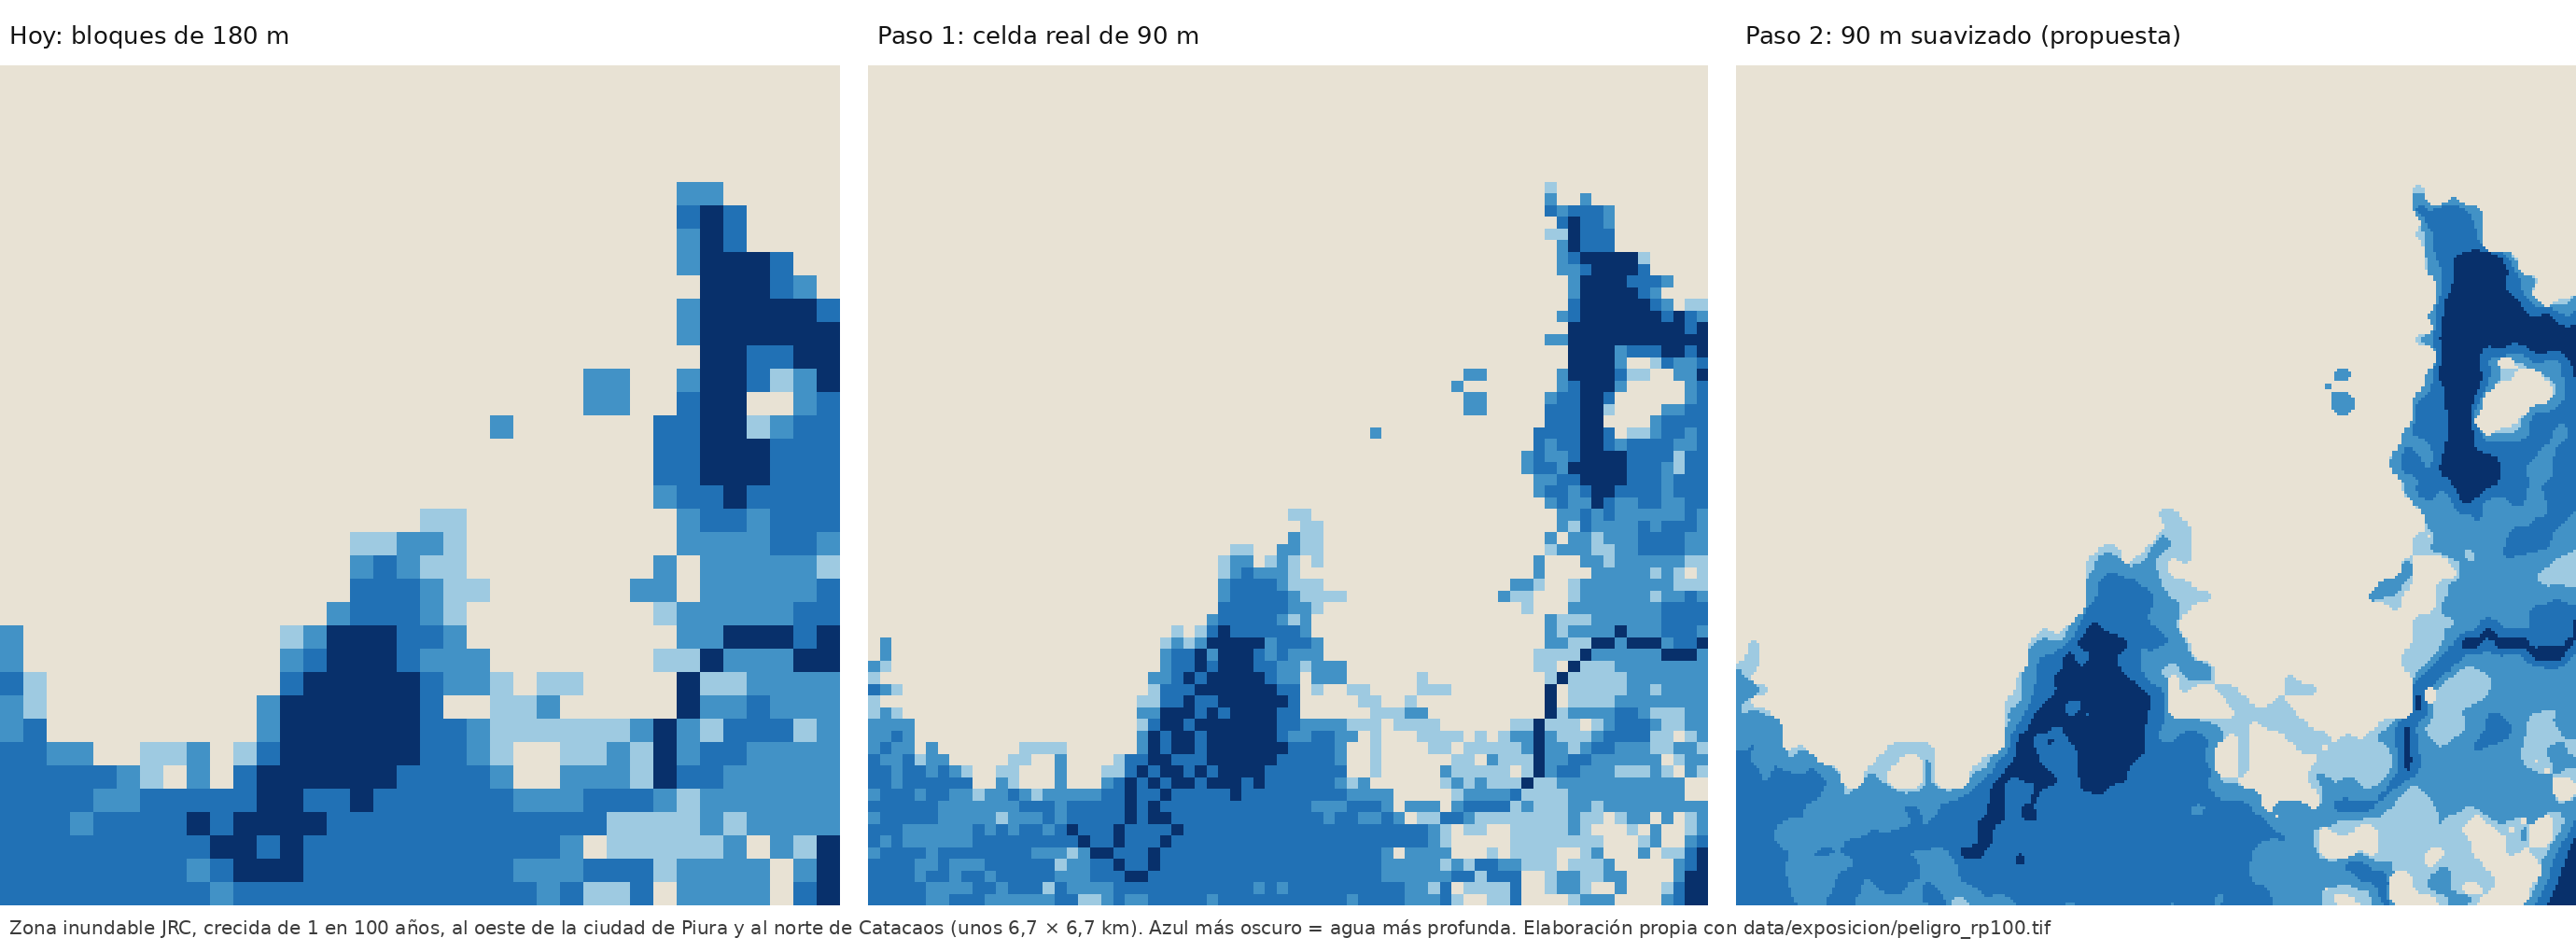
\includegraphics[width=\textwidth]{mapa_antes_despues.png}\\[2pt]
{\scriptsize\color{gris} La zona de 1 en 100 años cubre el 84,5 \% de lo inundado en Piura en 2017 (Copernicus EMSR199).}
\end{column}
\end{columns}
\end{frame}

% ---------------------------------------------------------------- 13
\begin{frame}{Cruce con los Censos Nacionales 2025}
\begin{columns}[T]
\begin{column}{0.36\textwidth}
\begin{caja}{Método}
\begin{enumerate}\footnotesize
\item Cada manzana se ubica por un punto interior; cada centro poblado, por su punto.
\item Se lee la profundidad del agua del JRC en ese punto.
\item Se suman viviendas y personas por distrito.
\end{enumerate}
\end{caja}
{\scriptsize Los datos por manzana no están en el repositorio. Solo se publican totales por distrito y nunca cifras menores de 10.}
\end{column}
\begin{column}{0.6\textwidth}\footnotesize
\begin{tabular}{@{}lrr@{}}\toprule
Censos Nacionales 2025 & 1 en 10 & 1 en 100\\\midrule
Viviendas & 77 718 & \textbf{109 602}\\
Personas & 290 735 & \textbf{407 877}\\
Niños de 0 a 4 años & — & 30 338\\
Personas de 65 años o más & — & 35 057\\
Mujeres & — & 207 303\\
Paredes de material frágil & — & 37 849 (35 \%)\\
Piso de tierra & — & 41 707 (38 \%)\\
Con más de 1,5 m de agua & — & 48 703\\\bottomrule
\end{tabular}\\[4pt]
En la zona de 1 en 100 años hay además \textbf{685 colegios} (124 497 alumnos) y \textbf{146 establecimientos de salud}. Es el 17 \% de la población de ambos departamentos.
\end{column}
\end{columns}
\end{frame}

\parte{3}{Confirmar: el radar satelital}

% ---------------------------------------------------------------- 15
\begin{frame}{Cómo el radar Sentinel-1 «ve» el agua}
\centering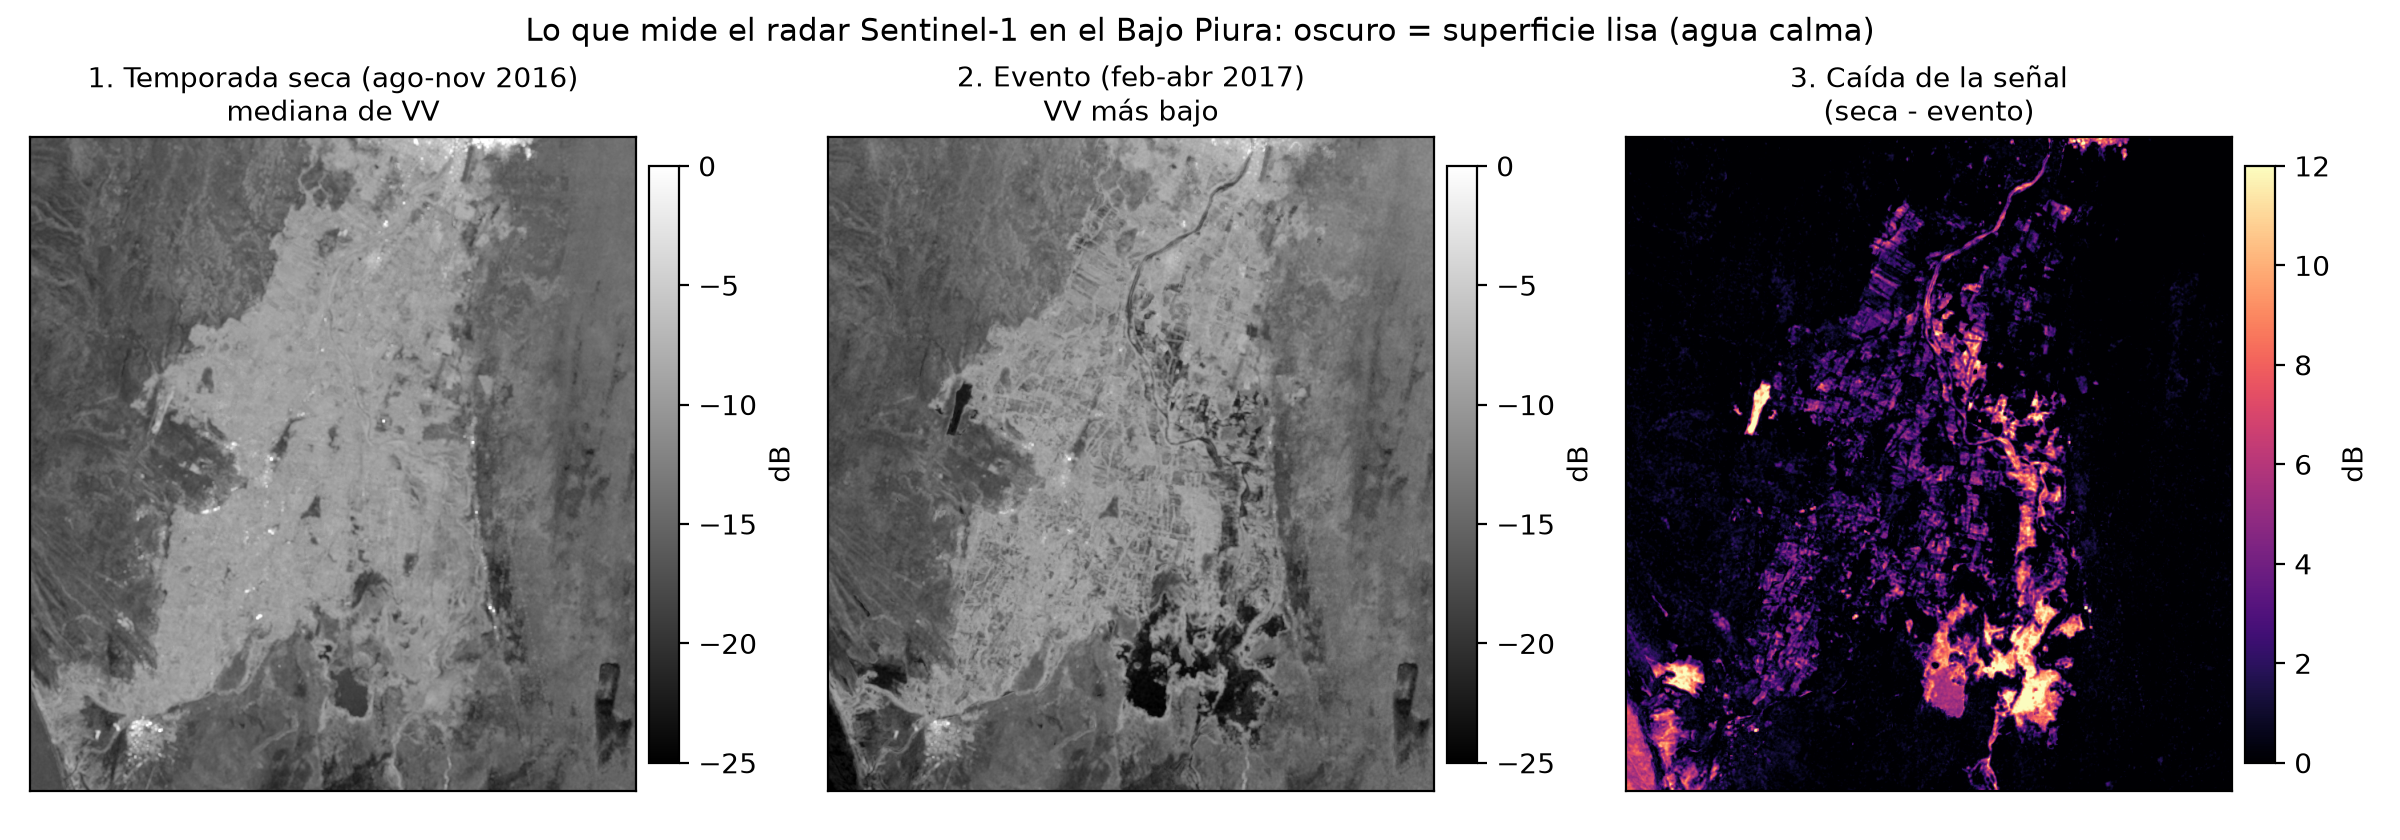
\includegraphics[width=0.92\textwidth]{agua_1_radar.png}\\[4pt]
\begin{columns}[T]
\begin{column}{0.48\textwidth}\small
El radar emite microondas y mide el eco ($\sigma^0_{VV}$, en dB). El agua calma refleja la señal lejos del satélite: se ve oscura. Funciona de noche y con nubes.
\end{column}
\begin{column}{0.48\textwidth}
\begin{cajasin}\centering
Un píxel está inundado si\\ $\sigma^0_{\text{evento}} < -17$ dB \quad y \quad $\sigma^0_{\text{seca}}-\sigma^0_{\text{evento}} > 3$ dB
\end{cajasin}
\end{column}
\end{columns}
\end{frame}

% ---------------------------------------------------------------- 16
\begin{frame}{Reglas para quitar falsas alarmas y validación con el mapa oficial}
\centering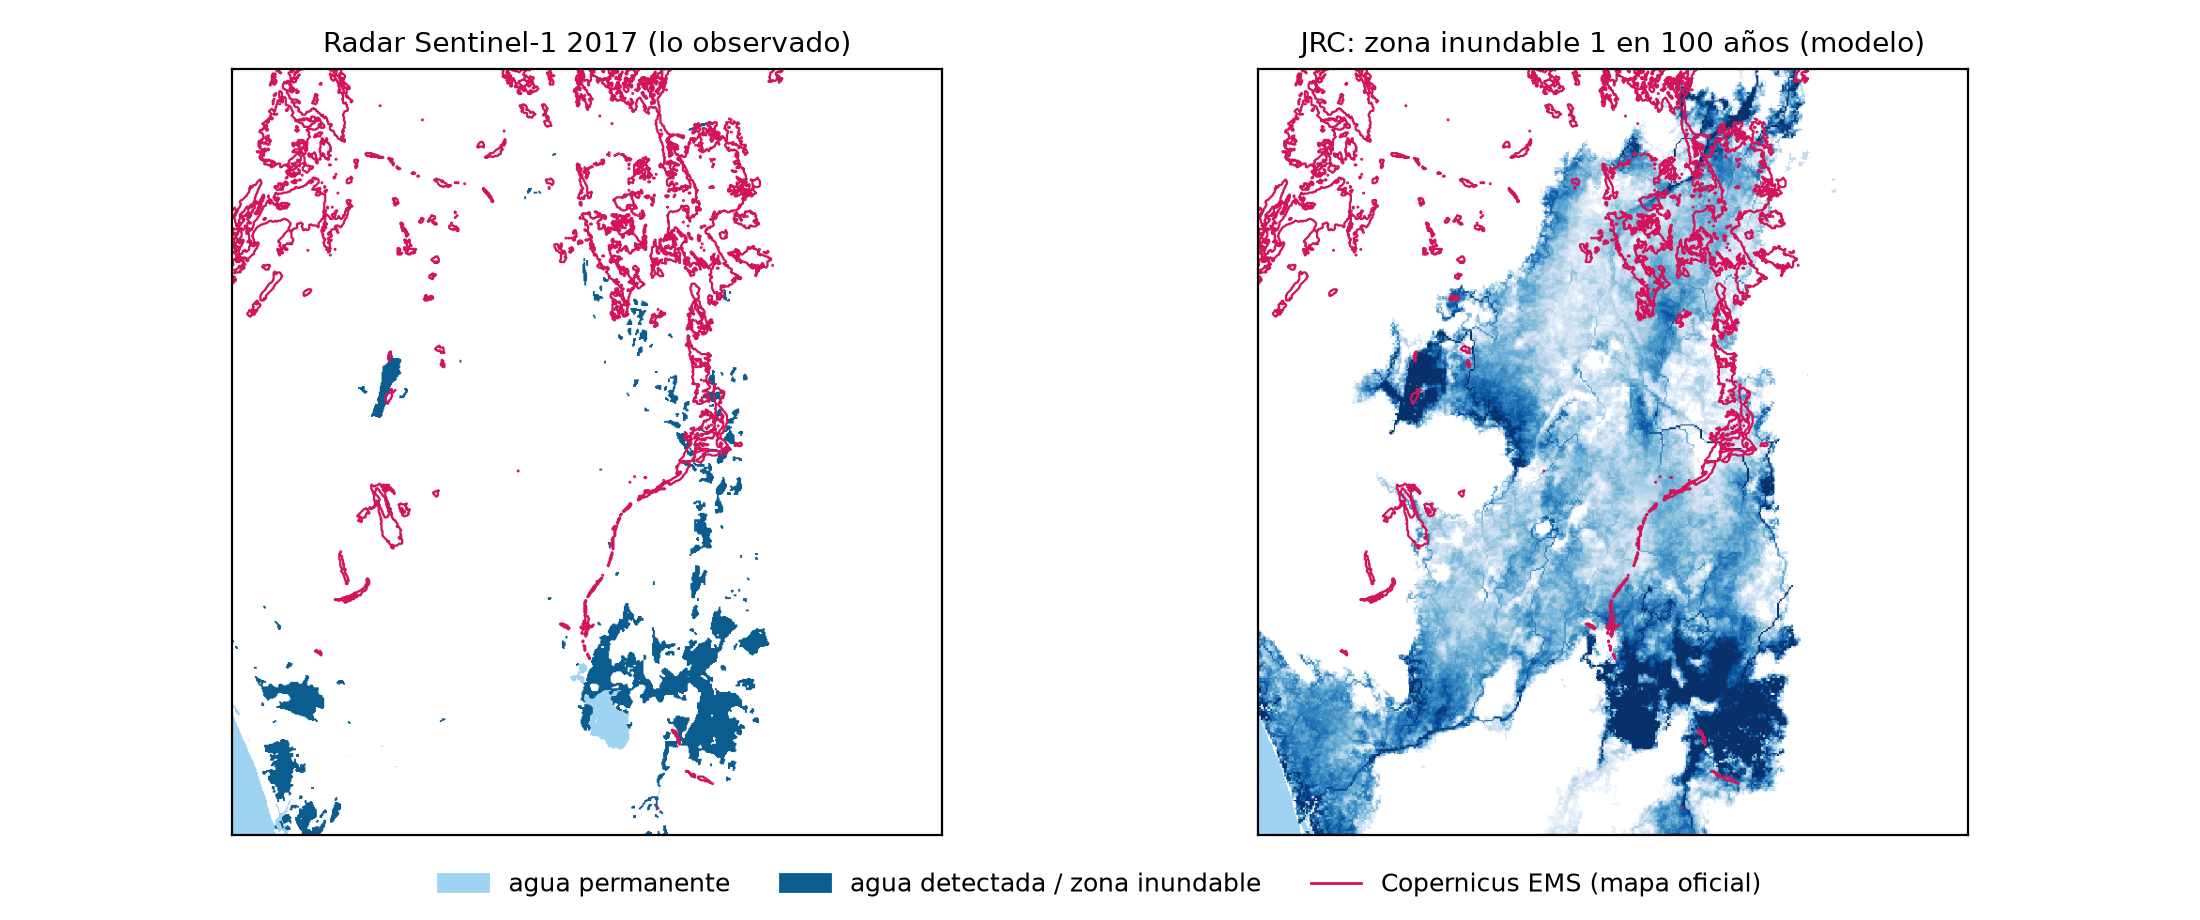
\includegraphics[width=0.66\textwidth]{agua_5_comparacion.png}\\[3pt]
\begin{columns}[T]
\begin{column}{0.48\textwidth}
\begin{caja}{Máscaras}
Se quita el agua permanente, lo que está a más de 250 m de altura, las pendientes mayores a 5° y las manchas de menos de 5 píxeles.
\end{caja}
\end{column}
\begin{column}{0.48\textwidth}
\begin{caja}[verde]{Frente a Copernicus EMS 2017}
El radar detectó el \textbf{41,7 \%} del área inundada y el \textbf{63,4 \%} de lo que marcó coincide. La zona JRC cubre el \textbf{84,5 \%}.
\end{caja}
\end{column}
\end{columns}
\end{frame}

% ---------------------------------------------------------------- 17
\begin{frame}{Por qué el radar no basta para anticipar}
\centering
\begin{tikzpicture}[font=\scriptsize]
\draw[-{Latex},thick] (0,0) -- (12.5,0) node[right]{días};
\foreach \x in {0,...,7} {\draw (1.5*\x,0.1) -- (1.5*\x,-0.1) node[below]{\x};}
\node[draw=azul,fill=azul!10,rounded corners,align=center] at (0,1.1) {Satélite pasa:\\seco};
\node[draw=azul,fill=azul!10,rounded corners,align=center] at (9,1.1) {Vuelve a pasar:\\seco otra vez};
\fill[rojo!25] (3,0.25) rectangle (6,0.75); \node at (4.5,0.5) {inundación (1–2 días)};
\node[color=rojo] at (4.5,1.2) {lluvia fuerte};
\draw[decorate,decoration={brace,mirror,amplitude=4pt},gris] (0,-0.6) -- (9,-0.6) node[midway,below=5pt]{el evento ocurrió entre dos pasadas};
\end{tikzpicture}
\par\vspace{0.6em}
\begin{columns}[T]
\begin{column}{0.48\textwidth}\begin{caja}[rojo]{Límites}
Pasa cada varios días · no ve el agua entre casas ni en la sierra · llega después del evento. Detectó solo 4 de 13 eventos de la prensa.
\end{caja}\end{column}
\begin{column}{0.48\textwidth}\begin{caja}[verde]{Decisión}
El radar se queda para \textbf{confirmar}. Para anticipar se usa lo que se sabe antes: lluvia, ríos, mar y época del año.
\end{caja}\end{column}
\end{columns}
\end{frame}

\parte{4}{Anticipar a corto plazo: el aviso de lluvia y caudal}

% ---------------------------------------------------------------- 19
\begin{frame}{Aviso de lluvia y caudal: los próximos 1 a 3 días}
\begin{columns}[T]
\begin{column}{0.5\textwidth}\small
Para cada distrito $d$ y día $j$, con el pronóstico de lluvia $\hat P_{d,j}$ (Open-Meteo):
\[\text{nivel}_{d,j}=\begin{cases}\text{extremo} & \text{si } \hat P_{d,j} > P_{99}(\text{provincia})\\ \text{fuerte} & \text{si } \hat P_{d,j} > P_{95}(\text{provincia})\\ \text{normal} & \text{en otro caso}\end{cases}\]
{\footnotesize $P_{95}$ y $P_{99}$: percentiles de los días con lluvia ($\ge 1$ mm) de 1991–2020 (ERA5). En los distritos ribereños el nivel también sube si el caudal pronosticado por GloFAS pasa su $P_{95}$ o $P_{99}$.}\par\vspace{6pt}
{\footnotesize\textbf{No es un aviso oficial:} los oficiales son de SENAMHI, ENFEN e INDECI.}
\end{column}
\begin{column}{0.46\textwidth}
\begin{caja}[verde]{Pronósticos reales}
\textbf{9 de 10} inundaciones recientes tuvieron aviso fuerte o extremo antes de ocurrir; 5 de ellas, con 3 días.
\end{caja}
\begin{caja}[verde]{24 años del SINPAD}
Una semana con aviso tiene entre \textbf{10 y 21 veces} más probabilidad de viviendas afectadas que una sin aviso.
\end{caja}
\begin{caja}[naranja]{Falsas alarmas}
El \textbf{42,9 \%} de los avisos de lluvia fue seguido de daño, frente al 18,4 \% al azar.
\end{caja}
\end{column}
\end{columns}
\end{frame}

\parte{5}{Anticipar semanas antes: el modelo}

% ---------------------------------------------------------------- 21
\begin{frame}{Planteamiento del modelo}
\begin{cajasin}\small
Para cada distrito $d$, cada semana $t$ y cada plazo $h=1,2,3,4$: estimar la \textbf{probabilidad} de que el INDECI registre una emergencia por lluvia o inundación \textbf{exactamente en la semana $t+h$}, con lo que se conoce al cerrar la semana $t$.
\end{cajasin}
\begin{columns}[T]
\begin{column}{0.22\textwidth}\cifra{78}{distritos (13 Tumbes, 65 Piura)}\end{column}
\begin{column}{0.22\textwidth}\cifra{1 200}{semanas (2003–2025)}\end{column}
\begin{column}{0.22\textwidth}\cifra{73 242}{filas de prueba por plazo (2008–2025)}\end{column}
\begin{column}{0.22\textwidth}\cifra[rojo]{3,1 \%}{semanas con emergencia}\end{column}
\end{columns}
\centering
\begin{tikzpicture}[font=\scriptsize]
\foreach \i/\l in {0/$t-3$,1/$t-2$,2/$t-1$,3/$t$,4/$t+1$,5/$t+2$,6/$t+3$,7/$t+4$}{
 \ifnum\i<4 \fill[azul!20] (1.35*\i,0) rectangle +(1.25,0.5); \else \fill[naranja!25] (1.35*\i,0) rectangle +(1.25,0.5); \fi
 \node at (1.35*\i+0.62,0.25) {\l};}
\node[color=azul] at (2.6,-0.35) {\textbf{X}: lo que ya se sabe};
\node[color=naranja] at (8,-0.35) {\textbf{Y}: una probabilidad para cada semana $t+h$};
\draw[thick,rojo] (5.35,-0.15) -- (5.35,0.75) node[above]{hoy};
\end{tikzpicture}
\end{frame}

% ---------------------------------------------------------------- 22
\begin{frame}{Variable dependiente Y: de dónde sale}
\begin{columns}[T]
\begin{column}{0.42\textwidth}\centering
\begin{tikzpicture}[font=\scriptsize]
\node[barra=70,minimum width=4.6cm,text=white] at (0,0) {SINPAD: todo el Perú \hfill 151 491};
\node[barra=55,minimum width=3.8cm,text=white] at (0,-0.62) {Solo Tumbes y Piura \hfill 8 556};
\node[barra=40,minimum width=3.0cm] at (0,-1.24) {Solo lluvia o inundación \hfill 3 363};
\node[barra=25,minimum width=2.6cm] at (0,-1.86) {Distrito-semanas \hfill 2 691};
\end{tikzpicture}\\[4pt]
\begin{caja}{SINPAD}
Registro oficial de emergencias del INDECI: fecha en que ocurrió, distrito, peligro y daños. No trae fecha de fin. Se publica cada seis meses.
\end{caja}
\end{column}
\begin{column}{0.54\textwidth}
\begin{cajasin}
\[E_{d,s}=\ind\Big[\textstyle\sum_r \ind(r\in d,\ r\in s,\ r \text{ de agua})\ge 1\Big]\]
\[Y^{(h)}_{d,t}=E_{d,\,t+h},\qquad h=1,\dots,4\]
\end{cajasin}
\small $Y=1$: hay al menos un registro de agua en la semana $t+h$. $Y=0$: ninguno. El 0 es la ausencia de registros nuevos.\\[4pt]
\footnotesize Antes, una sola $Y$ miraba las 4 semanas juntas ($\max_{k} E_{d,t+k}$). Ahora hay \textbf{una $Y$ por plazo}: así se sabe a cuántas semanas el modelo sí aporta.
\end{column}
\end{columns}
\end{frame}

% ---------------------------------------------------------------- 23
\begin{frame}{Y en los 78 distritos, de 2003 a 2025}
\centering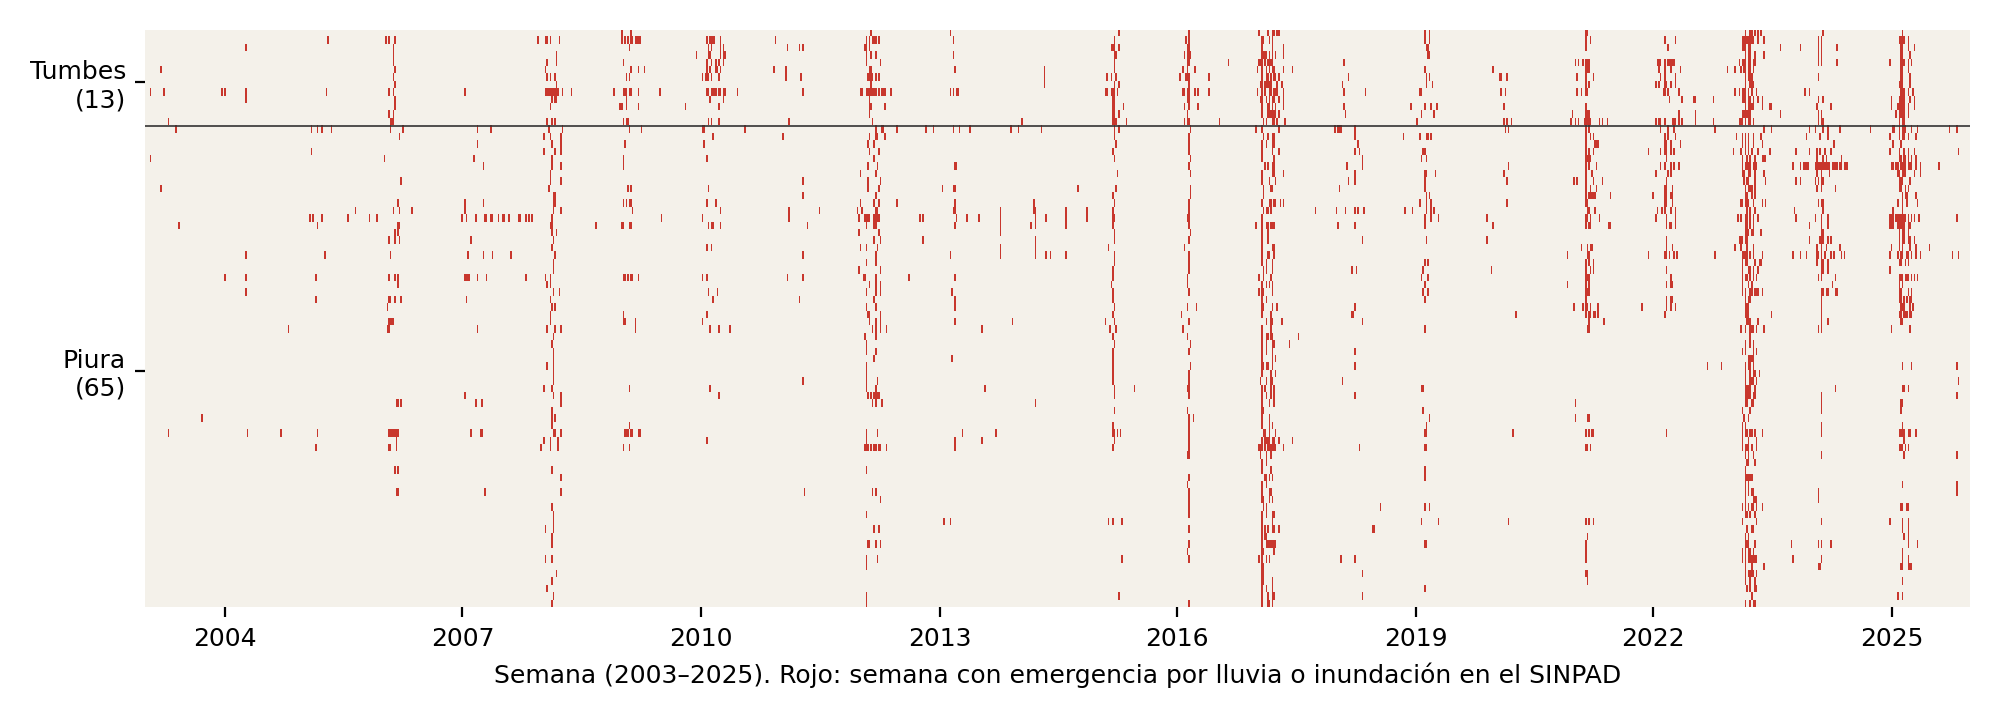
\includegraphics[width=\textwidth]{y_heatmap.png}
\begin{columns}[T]
\begin{column}{0.48\textwidth}\begin{itemize}\footnotesize
\item 2,6 \% de las distrito-semanas tienen emergencia (3,1 \% en 2008–2025).
\item \textbf{90 \%} de los registros, de enero a abril.
\end{itemize}\end{column}
\begin{column}{0.48\textwidth}\begin{itemize}\footnotesize
\item Picos: 2017 y 2023; también 2025.
\item El registro crece en los años recientes: se corrige al calibrar.
\end{itemize}\end{column}
\end{columns}
\end{frame}

% ---------------------------------------------------------------- 24
\begin{frame}{Variables independientes X: todas conocidas al cerrar la semana $t$}
\tiny
\begin{tabularx}{\textwidth}{@{}l l X@{}}
\toprule
\textbf{Grupo · fuente} & \textbf{Variable} & \textbf{Definición}\\\midrule
Lluvia · NASA POWER & log lluvia 30 d, log lluvia 7 d & Lluvia acumulada en 4 semanas y en la última semana\\
 & lluvia sobre p95, sobre p99 & ¿Algún día de la semana superó el percentil 95 o 99 del distrito?\\
Río · GloFAS & log caudal relativo & Caudal de la semana entre su mediana de esa semana del año\\
 & caudal sobre p95 & ¿El río superó su percentil 95 diario? (distritos ribereños)\\
Mar · NOAA & Niño 1+2 & Anomalía de temperatura del mar (°C)\\
Época · calendario & sen y cos de la semana objetivo & La semana $t+h$ como ángulo de un reloj\\
Historia · SINPAD & frecuencia histórica & Semanas con emergencia del distrito (solo años de entrenamiento)\\
Exposición · JRC y Censo & \% inundable, log viviendas, log personas & Área del distrito en zona de 1 en 100 años; viviendas y personas del censo en ella\\\bottomrule
\end{tabularx}\\[6pt]
\begin{caja}[naranja]{Lo que NO entra}
«¿Hubo emergencia esta semana?» se quitó: el SINPAD publica cada seis meses y ese dato no existe en tiempo real.
\end{caja}
\end{frame}

% ---------------------------------------------------------------- 25
\begin{frame}{Cómo se calcula cada variable}
\begin{columns}[T]
\begin{column}{0.56\textwidth}\small
\textbf{Lluvia de 30 días:} $L_{d,t}=\sum_{k=0}^{3}\text{lluvia}_{d,t-k}$, \quad $x_1=\log(1+L_{d,t})$\\[4pt]
\textbf{Día extremo:} $x=\ind\big[\max_{j\in t}\text{lluvia}_{d,j} > P_{95}(d)\big]$\\[4pt]
\textbf{Caudal relativo:} $x=\log\Big(\dfrac{Q_{r(d),t}}{\max\{\tilde Q_{r(d),w(t)},\,0{,}5\}}\Big)$\\[4pt]
\textbf{Historia:} $x=\dfrac{1}{|S_{\text{entreno}}|}\sum_{s\in S_{\text{entreno}}}E_{d,s}$\\[4pt]
\textbf{Época:} $\theta=2\pi\,\dfrac{w(t+h)}{52}$, \quad $\sin\theta$, $\cos\theta$
\end{column}
\begin{column}{0.4\textwidth}
\begin{caja}{¿Por qué logaritmo?}
Vuelve comparables los valores extremos de lluvia y caudal.
\end{caja}
\begin{caja}{¿Por qué seno y coseno?}
Así la semana 52 y la semana 1 quedan juntas, como las 11:59 y las 12:00.
\end{caja}
\begin{caja}[naranja]{Últimos días}
Los días que NASA POWER aún no publica se completan con Open-Meteo (provisionales).
\end{caja}
\end{column}
\end{columns}
\end{frame}

% ---------------------------------------------------------------- 26
\begin{frame}{El modelo: regresión logística + una segunda etapa para viviendas}
\begin{cajasin}\centering
$\Pr\big(Y^{(h)}_{d,t}=1\mid \mathbf{x}_{d,t}\big)=p_{d,t}=\dfrac{1}{1+\exp\!\big(-(\beta_0+\sum_j \beta_j z_{j,d,t})\big)}$,\qquad $z_j=\dfrac{x_j-\bar x_j}{s_j}$
\end{cajasin}
\small Los $\beta$ se estiman con penalización L2 ($C=0{,}3$) y \textbf{sin pesos de clase}, para que la salida se pueda leer como probabilidad:
\[\min_\beta\ -\sum_i\big[y_i\log p_i+(1-y_i)\log(1-p_i)\big]+\tfrac{1}{2C}\|\beta\|^2\]
\begin{caja}[verde]{Segunda etapa: ¿cuántas viviendas?}
$E[V\mid\mathbf{x}]=\underbrace{\Pr(V>0\mid\mathbf{x})}_{\text{logística}}\times\underbrace{E[V\mid V>0,\mathbf{x}]}_{\text{Gamma, enlace log}}$ \quad (como los modelos de impacto en dos etapas)
\end{caja}
\end{frame}

% ---------------------------------------------------------------- 27
\begin{frame}{Validación: cada año se predice con un modelo que nunca lo vio}
\centering
\begin{tikzpicture}[font=\scriptsize]
\foreach \y/\a/\n in {0/2008/1, -0.45/2009/2, -0.9/2010/3, -1.6/2017/9, -2.05/2025/17}{
 \fill[azul!35] (0,\y) rectangle (0.32*\n+1.2,\y+0.32);
 \fill[naranja!70] (0.32*\n+1.2,\y) rectangle (0.32*\n+1.52,\y+0.32);
 \node[anchor=west] at (7.2,\y+0.16) {probar \a};}
\node at (3,-1.15) {\dots}; \node at (3,0.6) {\color{azul}entrenar: semanas objetivo anteriores al 1 de enero del año de prueba};
\end{tikzpicture}
\par\vspace{0.4em}
\begin{columns}[T]
\begin{column}{0.52\textwidth}\small
\textbf{PR-AUC} $=\sum_n (R_n-R_{n-1})P_n$: combina precisión y exhaustividad; un modelo sin información saca la tasa (0,031).\\[3pt]
\textbf{BSS} $=1-\dfrac{\text{Brier}_{\text{modelo}}}{\text{Brier}_{\text{tasa media}}}$: calidad de la probabilidad.
\end{column}
\begin{column}{0.44\textwidth}
\begin{caja}{Referencias que hay que superar}
Climatología del distrito y su mes · mes del año · «hubo emergencia en $t$» · «llovió sobre p95 en $t$».
\end{caja}
{\scriptsize Exactitud no sirve: decir siempre «no» acierta el 97 \%.}
\end{column}
\end{columns}
\end{frame}

% ---------------------------------------------------------------- 28
\begin{frame}{Resultados por plazo (2008–2025)}
\begin{columns}[c]
\begin{column}{0.5\textwidth}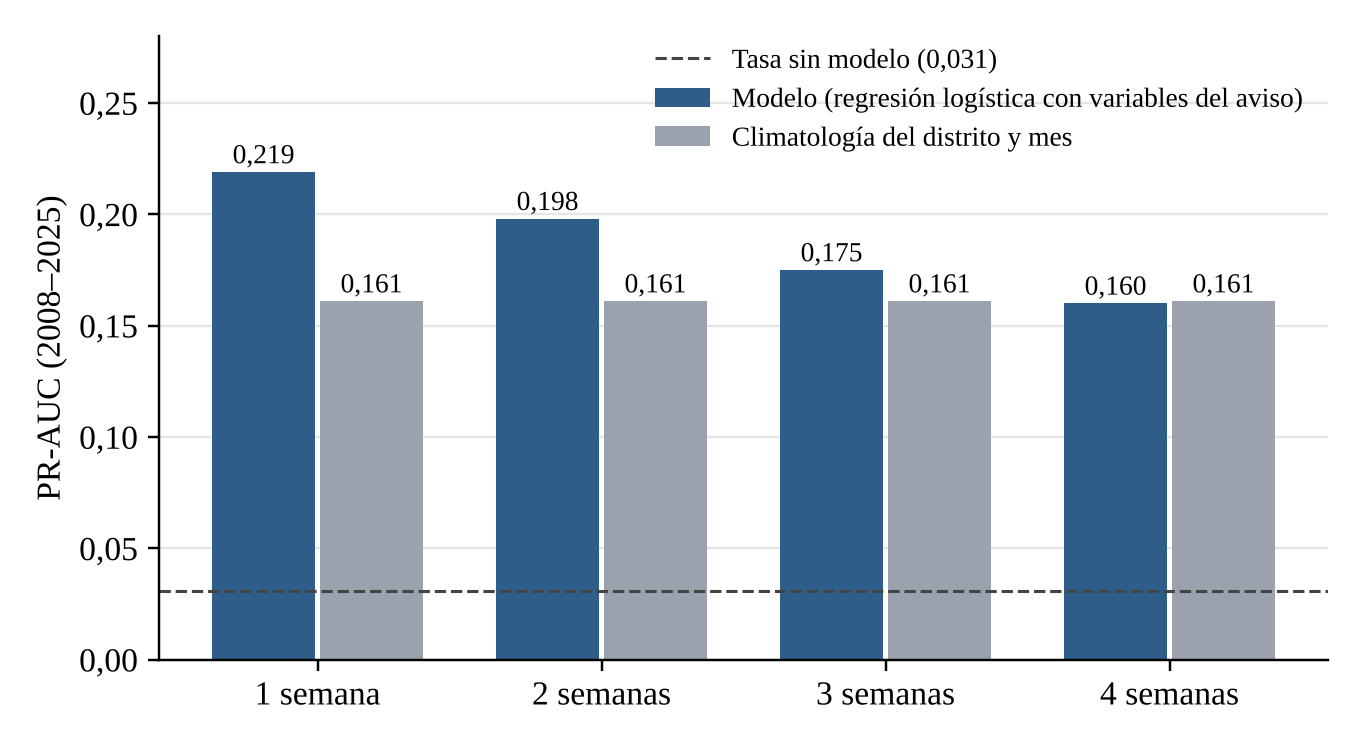
\includegraphics[width=\textwidth]{fig1_plazo.png}\end{column}
\begin{column}{0.47\textwidth}\tiny\setlength{\tabcolsep}{3pt}
\begin{tabular}{@{}lcccc@{}}\toprule
PR-AUC & 1 s & 2 s & 3 s & 4 s\\\midrule
\textbf{Logística} & \textbf{0,219} & \textbf{0,198} & 0,175 & 0,160\\
LightGBM & 0,229 & 0,204 & 0,186 & 0,165\\
Logística sin aviso & 0,206 & 0,188 & 0,170 & 0,163\\
Climatología & 0,161 & 0,161 & 0,161 & 0,161\\
Mes del año & 0,131 & 0,131 & 0,131 & 0,131\\
Tasa sin modelo & 0,031 & 0,031 & 0,031 & 0,031\\\bottomrule
\end{tabular}\\[5pt]
\begin{caja}[verde]{Lo logrado}
A una semana, \textbf{7 veces} la tasa y por encima de la climatología. La ventaja se reduce con el plazo y desaparece a 4 semanas.
\end{caja}
\end{column}
\end{columns}
\end{frame}

% ---------------------------------------------------------------- 29
\begin{frame}{¿La ventaja es real? Intervalos y test de realidad}
\begin{columns}[T]
\begin{column}{0.54\textwidth}\scriptsize
\setlength{\tabcolsep}{3.5pt}
\begin{tabular}{@{}lccc@{}}\toprule
Plazo & Modelo $-$ clim. & IC 95 \% & Gana (años)\\\midrule
1 semana & +0,058 & [0,024; 0,083] & 12 de 18\\
2 semanas & +0,037 & [0,008; 0,059] & 14 de 18\\
3 semanas & +0,014 & [$-$0,010; 0,033] & 9 de 18\\
4 semanas & 0,000 & [$-$0,019; 0,016] & 9 de 18\\\bottomrule
\end{tabular}\\[4pt]
Se sortean \textbf{años completos} 2 000 veces: las semanas de un mismo año no son independientes.
\end{column}
\begin{column}{0.42\textwidth}
\begin{caja}[naranja]{Test de realidad}
Si además se usan solo los datos de la semana anterior y umbrales calculados sin años futuros, la logística baja a \textbf{0,198} a una semana: sigue por encima de la climatología (0,161; IC [0,007; 0,058]).
\end{caja}
\begin{caja}[verde]{Conclusión}
Ventaja significativa a 1 semana (y a 2 en la versión publicada). A 3–4 semanas, empate.
\end{caja}
\end{column}
\end{columns}
\end{frame}

% ---------------------------------------------------------------- 30
\begin{frame}{Calibración: que «20 \%» signifique 20 \%}
\begin{columns}[T]
\begin{column}{0.5\textwidth}\small
\textbf{Calibración de Platt}, ajustada cada año solo con las predicciones fuera de muestra de los \textbf{cinco años anteriores}:
\[\text{logit}\,\tilde p = a + b\cdot\text{logit}\,p\]
No cambia el orden de las semanas; corrige el nivel. La causa principal: el SINPAD registra más en los años recientes.
\end{column}
\begin{column}{0.46\textwidth}\scriptsize
\begin{tabular}{@{}lcc@{}}\toprule
El modelo dijo & Ocurrió antes & Ocurrió después\\\midrule
5 a 10 \% & 12,4 \% & 8,5 \%\\
10 a 20 \% & 24,1 \% & 17,7 \%\\
20 a 30 \% & 28,8 \% & 26,1 \%\\
30 a 50 \% & 37,1 \% & 30,1 \%\\\midrule
Promedio / tasa real & 2,0 / 3,2 \% & \textbf{3,0 / 3,2 \%}\\\bottomrule
\end{tabular}\\[4pt]
{\color{gris}A una semana, 2010–2025. Por encima de 50 \% todavía exagera (120 casos).}
\end{column}
\end{columns}
\end{frame}

% ---------------------------------------------------------------- 31
\begin{frame}{Fases de aviso: atención y alerta}
\begin{columns}[T]
\begin{column}{0.48\textwidth}
\begin{caja}[naranja]{Atención: probabilidad $\ge$ 5 \%}
A una semana avisa antes de \textbf{7 de cada 10} emergencias; acierta 15 de cada 100 avisos; unos 8 avisos por distrito al año.
\end{caja}
\begin{caja}[rojo]{Alerta: probabilidad $\ge$ 15 \%}
Captura 35 \%; acierta \textbf{1 de cada 4} avisos (8 veces la tasa); unos 2 avisos por distrito al año.
\end{caja}
\end{column}
\begin{column}{0.48\textwidth}\scriptsize
\begin{tabular}{@{}lcccc@{}}\toprule
 & \multicolumn{2}{c}{Atención} & \multicolumn{2}{c}{Alerta}\\
Plazo & captura & precisión & captura & precisión\\\midrule
1 sem. & 70,6 \% & 15,1 \% & 35,1 \% & 25,5 \%\\
2 sem. & 71,2 \% & 14,0 \% & 26,1 \% & 22,1 \%\\
3 sem. & 68,5 \% & 13,0 \% & 22,1 \% & 19,3 \%\\
4 sem. & 66,6 \% & 12,1 \% & 19,7 \% & 18,1 \%\\\bottomrule
\end{tabular}\\[5pt]
\small Como los protocolos de acción temprana de la Cruz Roja: primero avisar con más falsas alarmas y actuar cuando hay más certeza.
\end{column}
\end{columns}
\end{frame}

% ---------------------------------------------------------------- 32
\begin{frame}{Práctica con años que el modelo nunca vio: 2017 y 2023}
\begin{columns}[c]
\begin{column}{0.54\textwidth}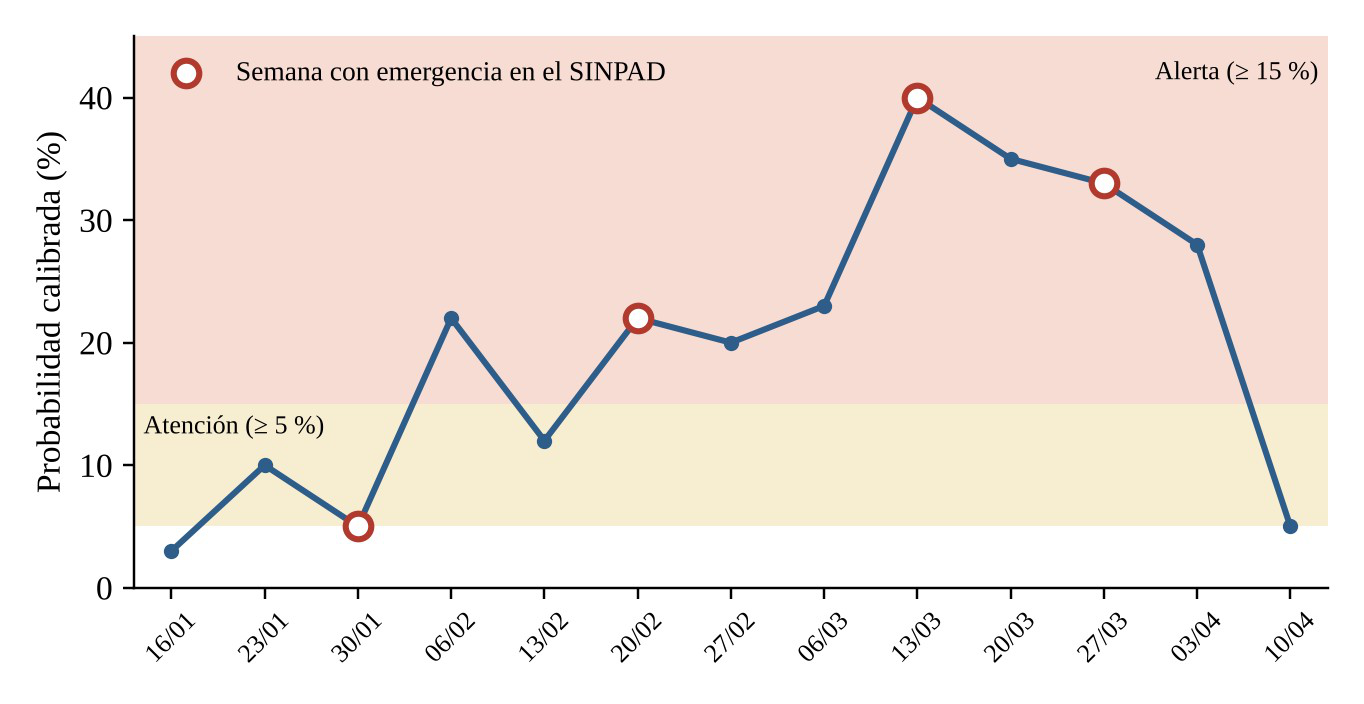
\includegraphics[width=\textwidth]{fig2_catacaos.png}\\
{\scriptsize\color{gris}Catacaos, 2017: probabilidad calculada la semana anterior; círculos = emergencia en el SINPAD.}\end{column}
\begin{column}{0.42\textwidth}\tiny\setlength{\tabcolsep}{3pt}
\begin{tabular}{@{}lcc@{}}\toprule
 & 2017 & 2023\\\midrule
Semanas con emergencia & 324 & 401\\
Con atención la semana antes & 82 \% & 76 \%\\
Con alerta & 52 \% & 36 \%\\
1.\textsuperscript{a} emergencia con aviso & 41 de 78 & 41 de 78\\\bottomrule
\end{tabular}\\[5pt]
\begin{caja}[naranja]{Lo más difícil}
La primera emergencia de cada distrito en la temporada.
\end{caja}
\end{column}
\end{columns}
\end{frame}

% ---------------------------------------------------------------- 33
\begin{frame}{Segunda etapa: ¿cuántas viviendas afectadas?}
\begin{columns}[T]
\begin{column}{0.5\textwidth}\small
Si ocurre la emergencia, una regresión \textbf{Gamma} estima cuántas viviendas se afectarían. Las viviendas esperadas son la probabilidad por esa cantidad.
\begin{caja}[rojo]{Subestima los años extremos}
Total estimado frente a lo registrado: \textbf{35 \% menos en 2017} y \textbf{66 \% menos en 2023}. Esos años tienen pocos antecedentes parecidos.
\end{caja}
\end{column}
\begin{column}{0.46\textwidth}
\begin{caja}[verde]{Cómo usarlo}
Para dimensionar la respuesta: la \textbf{exposición del censo} como techo y la \textbf{estimación del modelo} como piso.
\end{caja}
\begin{caja}{Ya está en el tablero}
Viviendas y personas «si ocurre», con el rango histórico del distrito (percentiles 10 y 90).
\end{caja}
\end{column}
\end{columns}
\end{frame}

\parte{6}{El producto: la temporada 2026}

% ---------------------------------------------------------------- 35
\begin{frame}{La temporada 2026, al 9 de noviembre}
\centering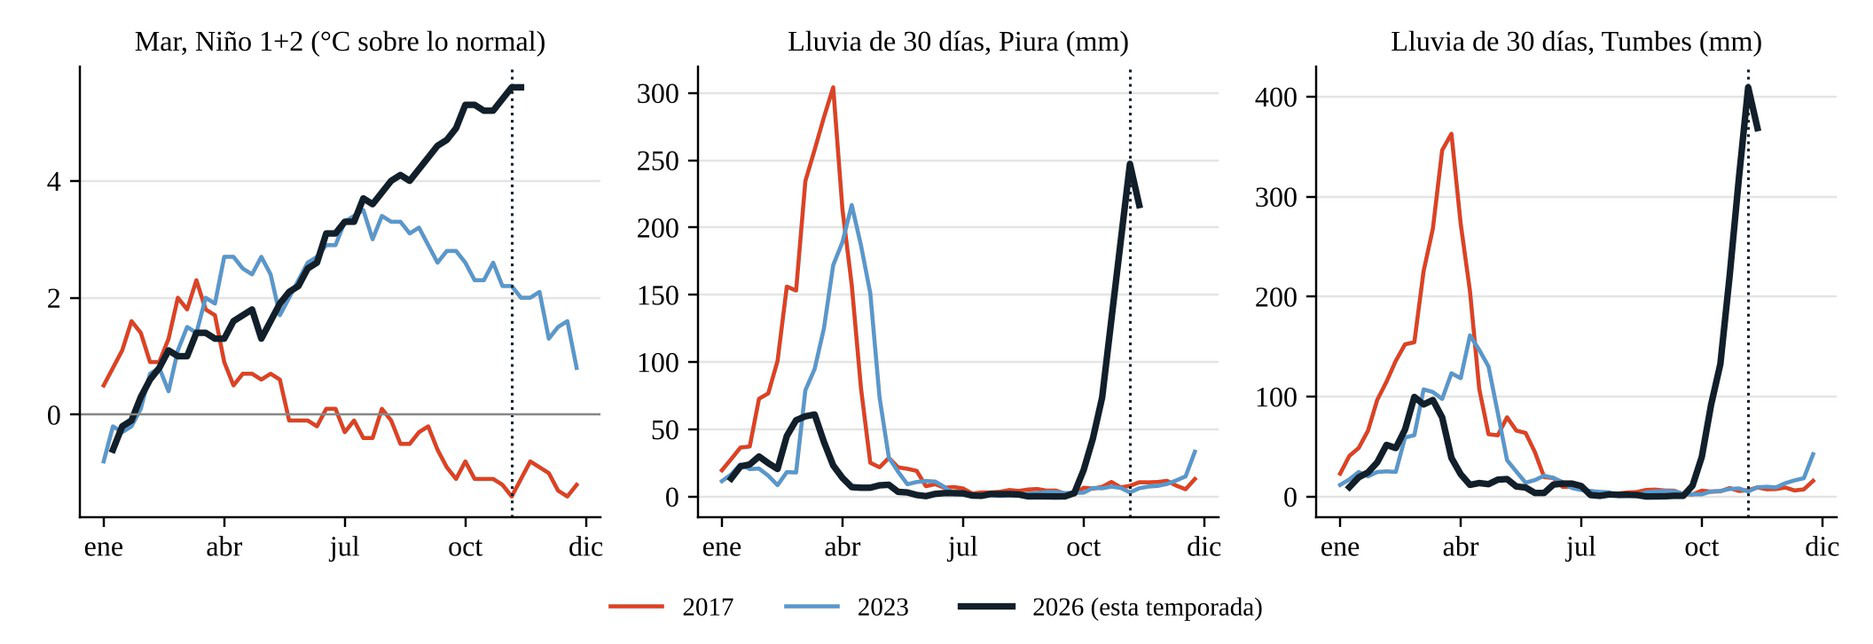
\includegraphics[width=0.78\textwidth]{fig3_2026.png}\\[2pt]
\scriptsize
\begin{tabular}{@{}lccc@{}}\toprule
Semana 45 del año (2 al 8 de noviembre) & 2017 & 2023 & \textbf{2026}\\\midrule
Niño 1+2 (°C sobre lo normal) & $-$1,4 & +2,2 & \textbf{+5,6}\\
Lluvia de 30 días, Piura / Tumbes (mm) & 8 / 6 & 3 / 5 & \textbf{247 / 409}\\
Caudal del río Piura (veces lo normal) & 1,2 & 0,8 & \textbf{8,5}\\\bottomrule
\end{tabular}
\end{frame}

% ---------------------------------------------------------------- 36
\begin{frame}{¿Dónde actuar primero? Probabilidad × personas expuestas}
\begin{columns}[c]
\begin{column}{0.34\textwidth}\centering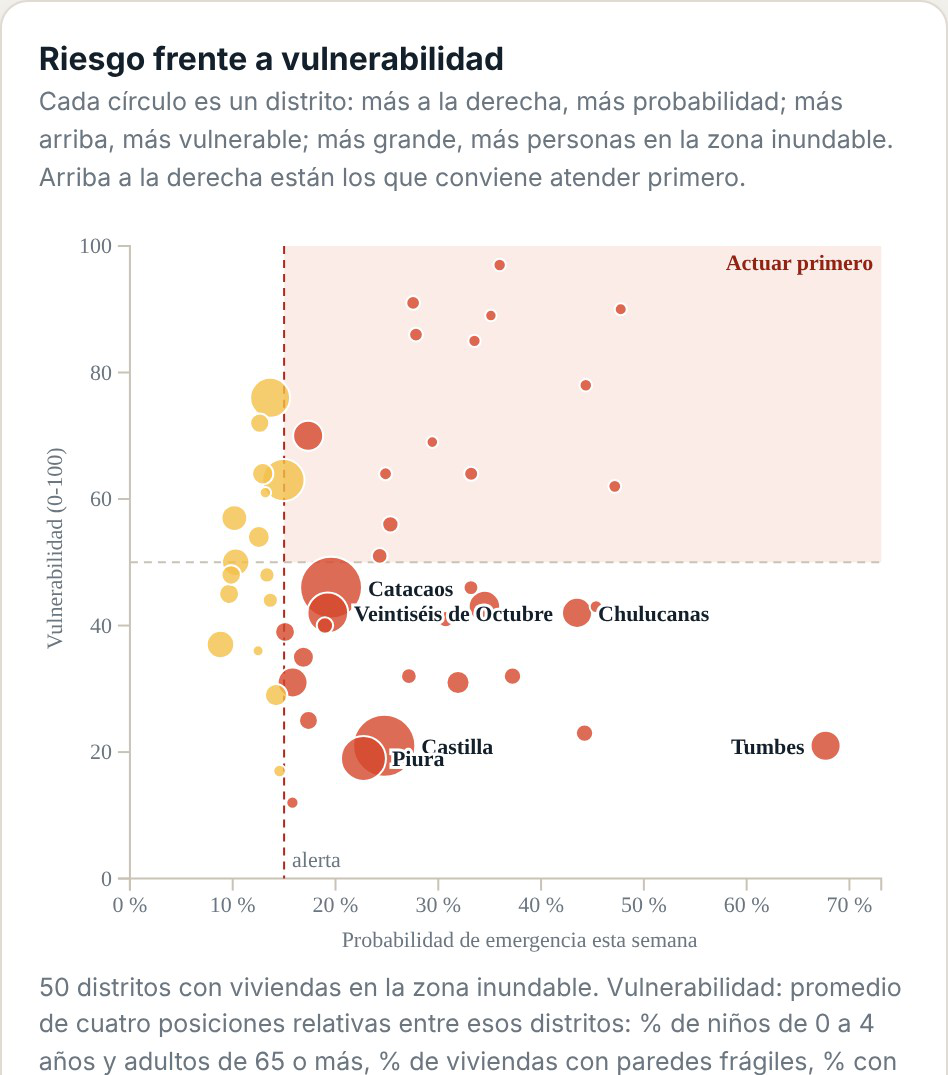
\includegraphics[height=0.7\textheight]{fig4_riesgo_vuln.png}\end{column}
\begin{column}{0.63\textwidth}\footnotesize
Semana del 9 al 15 de noviembre: \textbf{62 de 78} distritos en alerta y 16 en atención.
\[\text{riesgo esperado}_d = p_d \times \text{personas en zona inundable}_d\]
\begin{itemize}\footnotesize
\item Encabezan \textbf{Castilla} (25 \%, 78 961 expuestas), \textbf{Catacaos} (20 \%, 77 937) y \textbf{Piura} (23 \%, 35 430).
\item Tumbes tiene la probabilidad más alta (68 \%) pero menos gente expuesta.
\item Los 10 primeros concentran el 85 \% del riesgo esperado.
\end{itemize}
\begin{caja}[naranja]{Con cautela}
El mar (+5,6 °C) supera todo lo visto en el entrenamiento (máx. 3,5 °C): estas probabilidades son una extrapolación.
\end{caja}
\end{column}
\end{columns}
\end{frame}

% ---------------------------------------------------------------- 37
\begin{frame}{El tablero público}
\begin{columns}[c]
\begin{column}{0.5\textwidth}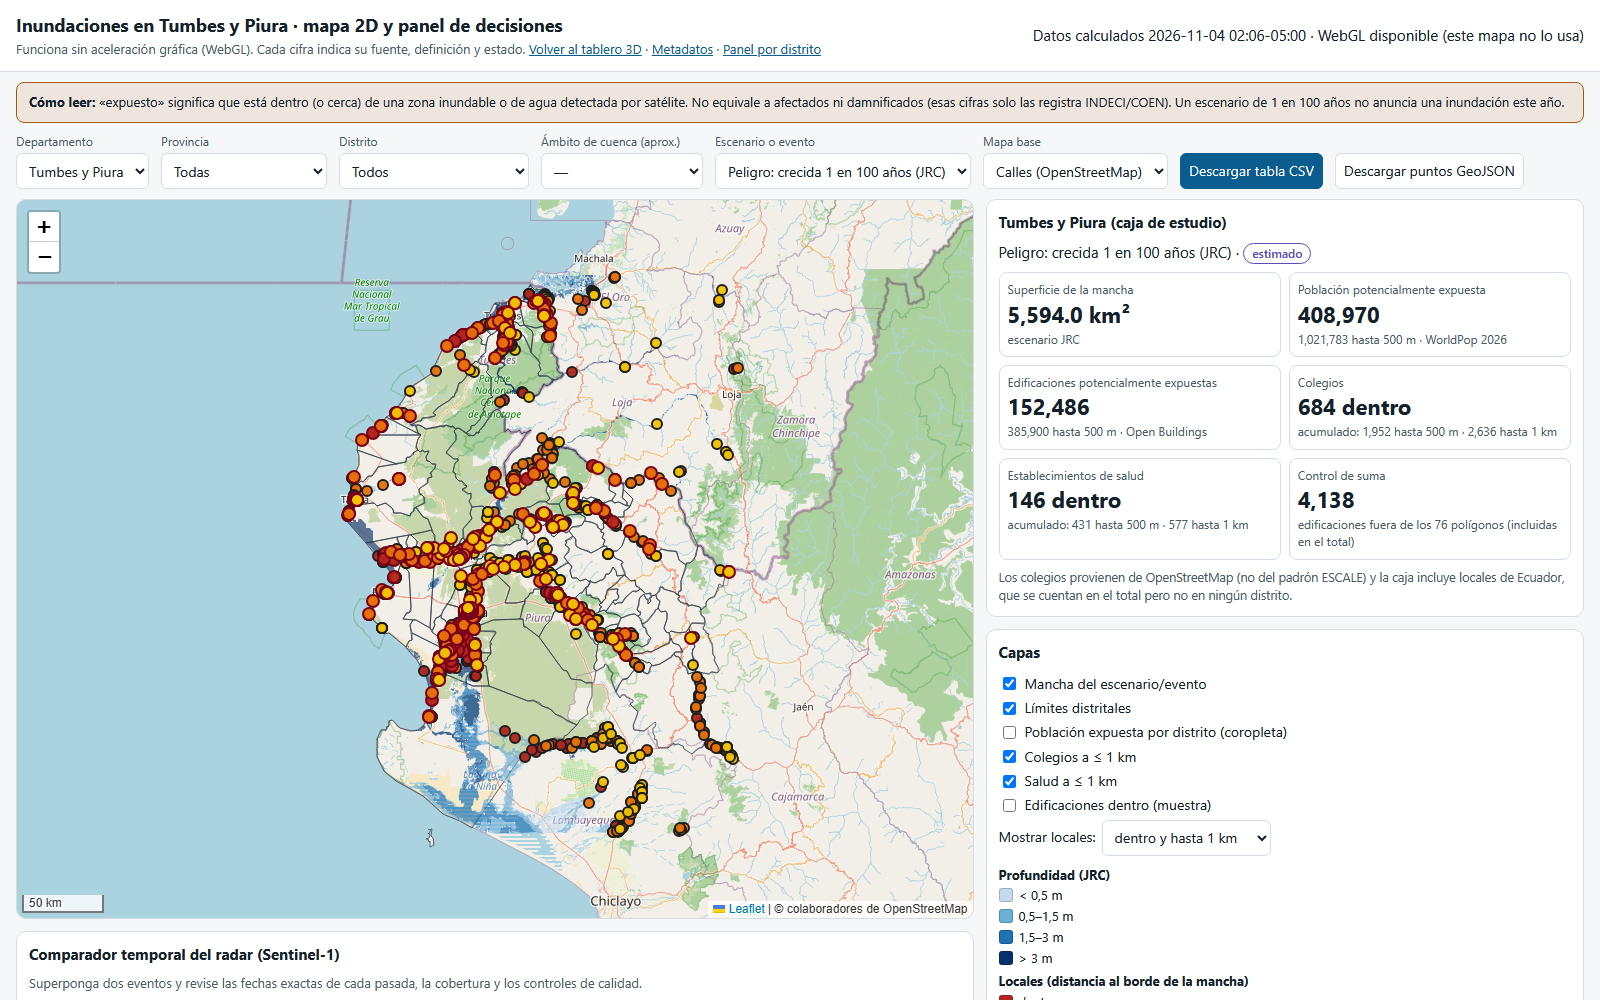
\includegraphics[width=\textwidth]{captura_mapa2d.png}\end{column}
\begin{column}{0.46\textwidth}
\begin{enumerate}\footnotesize
\item \textbf{Resumen:} cifras y estado del ENFEN.
\item \textbf{Mapa de inundación:} zona inundable, radar, viviendas, colegios y salud.
\item \textbf{Antes y después:} fotos Sentinel-2.
\item \textbf{Alerta por distrito:} probabilidad a 1–4 semanas, fases y por qué.
\item \textbf{¿Dónde actuar primero?} riesgo esperado y vulnerabilidad.
\item \textbf{Lluvia y ríos} frente a lo normal.
\item \textbf{El mar y El Niño:} 2026 frente a 2017 y 2023.
\item \textbf{Método y fuentes.}
\end{enumerate}
{\scriptsize maykolramirez.github.io/FENOMENO-PREDI}
\end{column}
\end{columns}
\end{frame}

% ---------------------------------------------------------------- 38
\begin{frame}{Cómo se comprobó todo}
\scriptsize
\begin{tabularx}{\textwidth}{@{}l X l@{}}\toprule
\textbf{Qué} & \textbf{Contra qué} & \textbf{Resultado}\\\midrule
Radar 2017 & Mapa oficial Copernicus EMS (EMSR199) & 41,7 \% detectado; 63,4 \% coincide\\
Zona inundable & Mismo mapa oficial 2017 & cubre el 84,5 \%\\
Exposición & Afectados del INDECI 2003–2024 por distrito & $\rho$ de Spearman 0,41\\
Aviso de lluvia & Pronósticos reales antes de 10 eventos & 9 de 10 avisados\\
Falsas alarmas & Todos los días de ene–abr 2025 y oct–nov 2026 & 42,9 \% vs. 18,4 \% al azar\\
Modelo & Validación año por año 2008–2025 & 0,219 vs. 0,161 (clim.) a 1 semana\\
Incertidumbre & Remuestreo por bloques de años & IC 95 \% [0,024; 0,083]\\
Robustez & Test de realidad (datos con retraso) & 0,198: sigue ganando a 1 semana\\
Código & 87 pruebas automáticas & 86 pasan, 1 omitida\\\bottomrule
\end{tabularx}\\[6pt]
\small Cada resultado tiene su programa en \texttt{herramientas/pruebas/} y su salida en \texttt{docs/evidencia/}: cualquiera puede repetirlo.
\end{frame}

% ---------------------------------------------------------------- 39
\begin{frame}{Limitaciones que reconocemos}
\begin{columns}[T]
\begin{column}{0.48\textwidth}
\begin{caja}{Datos}
\begin{itemize}\footnotesize
\item El SINPAD mide lo \textbf{registrado}: el registro creció con los años y se publica cada seis meses.
\item Lluvia en celdas de unos 50 km; PISCO diario solo es público hasta 2016–2018.
\item El mapa JRC no considera diques ni la inundación urbana por lluvia.
\end{itemize}
\end{caja}
\end{column}
\begin{column}{0.48\textwidth}
\begin{caja}[naranja]{Métodos}
\begin{itemize}\footnotesize
\item A 3–4 semanas el modelo no supera a la climatología.
\item La primera emergencia de la temporada es la más difícil (41 de 78).
\item Subestima las viviendas en años extremos.
\item 2026 está fuera del rango de entrenamiento (+5,6 °C).
\item Expuesto no es afectado; los avisos no son oficiales.
\end{itemize}
\end{caja}
\end{column}
\end{columns}
\end{frame}

% ---------------------------------------------------------------- 40
\begin{frame}{Aporte y próximos pasos}
\begin{columns}[T]
\begin{column}{0.48\textwidth}
\begin{caja}[verde]{Aporte para el INEI}
\begin{itemize}\footnotesize
\item Pasa de «cuántos viven en el distrito» a «cuántos viven donde el agua llega y qué tan probable es que llegue».
\item Une el Censo 2025 con el riesgo por distrito, sexo y edad.
\item Indicador semanal reproducible, con código abierto.
\item Solo totales por distrito; ninguna cifra menor de 10.
\end{itemize}
\end{caja}
\end{column}
\begin{column}{0.48\textwidth}
\begin{caja}{Próximos pasos}
\begin{enumerate}\footnotesize
\item Tablas de exposición del censo para todo el país.
\item Lluvia de mayor resolución (CHIRPS o PISCO).
\item Caudal pronosticado (re-pronósticos de GloFAS) para 3–4 semanas.
\item Registro del SINPAD más oportuno, con el INDECI.
\item Prueba prospectiva: guardar las predicciones de enero a abril de 2027 y compararlas con lo que pase.
\end{enumerate}
\end{caja}
\end{column}
\end{columns}
\end{frame}

% ---------------------------------------------------------------- 41
{\setbeamertemplate{footline}{}\setbeamercolor{background canvas}{bg=azul}
\begin{frame}\color{white}\vspace{2em}
{\Large\bfseries En resumen}\par\vspace{0.5em}{\color{naranja}\rule{4em}{2pt}}\par\vspace{0.8em}
\small Con datos públicos y del censo, estimamos la probabilidad de emergencia por distrito con una ventaja significativa sobre la historia del distrito a una semana, la convertimos en fases de aviso y la cruzamos con las personas expuestas del Censo 2025 para decidir dónde actuar primero.\par\vspace{1.5em}
{\Large\bfseries Gracias. ¿Preguntas?}\par\vspace{1em}
{\scriptsize maykolramirez.github.io/FENOMENO-PREDI · github.com/MaykolRamirez/FENOMENO-PREDI}
\end{frame}}

\end{document}
